\section{Yule過程}\label{s1:Yule過程} %{

\begin{procedure}\label{pro:Yule過程}
	任意の時刻$t\in\sizen_+$で必ず一つ新規スピシーズを作り、次の規則で
	ジーナスに追加する。
	\begin{enumerate} %{
		\item 確率$p_\new(t)$で新規ジーナスを作り、そのジーナスに新規スピシーズ
		を追加する。
		\item 確率$p_\new(t)^c$で既存のスピシーズをランダムに選び、その
		スピシーズの属するジーナスに新規スピシーズを追加する。
	\end{enumerate} %}
	ここで、任意の確率$p$に対して$p^c:=1-p$と定義する。
	\EOP
\end{procedure}

時刻$t$での関数$\nu_n(t)$と$\nu(t)$を次のように定義する。
\begin{itemize} %{
	\item 任意の$n\in\sizen$に対して$\nu_n(t)$をスピシーズを$n$個持つジーナス
	の数とする。任意の時刻で$\nu_0(t)=0$が成り立つ。
	\item $\nu(t)$をジーナスの総数とする。任意の時刻$t$で
	$\nu(t)=\sum_{n\in\sizen}\nu_n(t)$が成り立つ。
\end{itemize} %}
定義から時刻$t\in\sizen$でのスピシーズの総数は$t$となり、
$t=\sum_{n\in\sizen}n\nu_n(t)$が成り立つ。

保持するスピシーズの数をジーナスの状態とみなすと、ジーナスの状態変化は
次の状態遷移図で表すことができる。
\begin{equation*}\xymatrix{
	\ar[r]^{p_\new} 
	& 1 \ar[r]^{p_\new^c\cfrac{1}{t}} 
	& 2 \ar[r]^{p_\new^c\cfrac{2}{t}} 
	& 3 \ar[r]^{p_\new^c\cfrac{3}{t}} & \cdots
}\end{equation*}
任意の時刻$t$の関数$f(t)$に対して$\delta f(t):=f(t+1)-f(t)$とおくと、
$\nu_n(t)$は次の漸化式を満たす。
\begin{equation}\begin{split}\label{eq:delta-nu}
	\delta\nu_1(t+1) &= p_\new(t) - p_\new(t)^c\frac{1}{t}\nu_1(t) \\
	\delta\nu_{n+1}(t+1) &= p_\new(t)^c\frac{n}{t}\nu_n(t) 
		- p_\new(t)^c\frac{n+1}{t}\nu_{n+1}(t) 
		\quad\text{for all } n\in\sizen_+ \\
\end{split}\end{equation}
ここで、$\nu_n(t)$の生成関数$\nu(t,x)$を次のように定義すると、
\begin{equation}\begin{split}\label{eq:def-nu-1}
	\nu(t,x) := \sum_{n\in\sizen_+}\nu_n(t)x^n
\end{split}\end{equation}
漸化式\eqref{eq:delta-nu}は次の微分方程式で書き直すことができる。
\begin{equation}\begin{split}\label{eq:delta-nu-x}
	\delta\nu(t,x) = p_\new(t)x + \frac{p_\new(t)^c}{t}(x - 1)x\partial_x\nu(t,x)
\end{split}\end{equation}
生成関数$\nu(t,x)$を使うと、定義\eqref{eq:def-nu-1}から、
ジーナスの総数$\nu(t)$とスピシーズの総数$t$は次のように書け、
\begin{equation*}\begin{array}{rclcl}
	\nu(t) &=& \nu(t,1) &=& \sum_{n\in\sizen_+}\nu_n(t) \\
	t &=& \partial_x\nu(t,1) &=& \sum_{n\in\sizen_+}n\nu_n(t) \\
\end{array}\end{equation*}
それらの時間遷移は次のように書ける。
\begin{equation}\label{eq:nu-delta}\begin{array}{rclclcl}
	\delta\nu(t) &=& p_\new(t) \\
	\delta t &=& p_\new(t) + \cfrac{p_\new(t)^c}{t}\partial_x\nu(t,1)
	&=& p_\new(t) + p_\new^c(t) &= 1
\end{array}\end{equation}

時刻$t$でのジーナスの確率分布$\rho(t,x)$を次のように定義すると、
\begin{equation}\label{eq:def-rho-1}
	\rho(t,x) := \frac{\nu(t,x)}{\nu(t)}
\end{equation}
\eqref{eq:nu-delta}を使って、\eqref{eq:delta-nu-x}は次のように書ける。
\begin{equation}\label{eq:exact-rho}
	\rho(t+1,x) + \frac{\nu(t)}{p_\new(t)}\delta\rho(t,x) 
	= x + \frac{\nu(t)}{p_\new(t)}\frac{p_\new(t)^c}{t}
	(x - 1)x\partial_x\rho(t,x)
\end{equation}
ここで、時刻が無限大の極限で次の条件が成り立つと仮定する。
\begin{enumerate}\label{item:stable} %{
	\item\label{item:lhs} 次の式が成り立つ。
	\begin{equation*}
		\lim_{t\to\infty}\frac{\nu(t)}{p_\new(t)}\delta\rho(t,x) = 0
	\end{equation*}
	%
	\item\label{item:beta} ある$0<\beta\in\jitu\cup\set{\infty}$があって、
	次の式が成り立つ。
	\begin{equation}\label{eq:def-beta}
		\lim_{t\to\infty}\frac{\nu(t)}{p_\new(t)}\frac{p_\new(t)^c}{t} 
		= \frac{1}{\beta}
	\end{equation}
\end{enumerate} %}
条件\ref{item:lhs}は、次のように、ジーナスの確率分布が定常状態に収束するため
の十分条件になっている。
\begin{equation*}
	\delta\rho(t,x) = \frac{p_\new(t)}{\nu(t)}\frac{\nu(t)}{p_\new(t)}\delta\rho(t,x)
	\le \frac{\nu(t)}{p_\new(t)}\delta\rho(t,x)
	\quad\because\; \frac{p_\new(t)}{\nu(t)}\le 1 \quad\text{for all } 1\le t
\end{equation*}
これらの条件が成り立つと仮定し、時刻無限大の極限値を次のようにおくと、
\begin{equation}\label{eq:def-rho-2}
	\rho(x) := \lim_{t\to\infty}\rho(t,x)
\end{equation}
微分方程式\eqref{eq:delta-nu-x}の時刻が無限大の極限は次のようになる。
\begin{equation}\label{eq:diff-rho}
	\rho(x) = x + \frac{1}{\beta}(x - 1)x\partial_x\rho(x)
\end{equation}

$\rho(x)$を原点周りで次のようにべき展開\eqref{eq:def-rho-2}し、微分方程式
\eqref{eq:diff-rho}に代入すると、
\begin{equation}\label{eq:rho-taylor}
	\rho(x) = \sum_{n\in\sizen}\rho_nx^n
\end{equation}
次の漸化式が得られる。
\begin{equation*}
	\rho_0 = 0,\quad \rho_1 = \frac{\beta}{\beta + 1},\quad
	\rho_{n + 2} = \frac{n + 1}{\beta + n + 2}\rho_{n + 1}
	\quad\text{for all } n\in\sizen
\end{equation*}
この漸化式を解くと次のようになり、
\begin{equation}\label{eq:rho-taylor}
	\rho_0 = 0,\quad \rho_{n + 1} = \beta B(n + 1, \beta + 1)
	\quad\text{for all } n\in\sizen
\end{equation}
微分方程式\eqref{eq:diff-rho}の解$\rho(\beta|x)$は積分の形で次のように
求まる。
\begin{equation}\label{eq:rho-int}
	\rho(\beta|x) = \beta\int_0^1 dt \frac{(1 - t)^\beta}{1 - xt}
	\quad\text{for all } x\in\blr{-\infty, 1}
\end{equation}

微分方程式\eqref{eq:diff-rho}の解には積分定数が含まれるはずだが、原点近傍で
Taylor展開\eqref{eq:rho-taylor}を持つ解は\eqref{eq:rho-int}に限られる。
また、$\rho_n$が確率分布になっているという条件$\rho(1)=1$が、微分方程式
\eqref{eq:diff-rho}の解への境界条件になり、$\rho(1)=1$を満たす解は
\eqref{eq:rho-int}だけになることがわかる。したがって、定常状態に収束するため
の十分条件\ref{item:stable}が満たされるならば、その定常状態は$\beta$の値のみ
に依存して、唯一つ\eqref{eq:rho-int}に定まるという際立った性質を持っている。

ジーナスが平均でスピシーズを幾つ持つかは$\sum_{n\in\sizen}n\rho_n$で
表されるが、$x$が大きく$y$が固定されている時のベータ関数の近似
$B(x,y)\sim\Gamma(y)x^{-y}$を用いると、次のようになり、
\begin{equation*}
	\sum_{n\in\sizen}n\rho_n \sim \Gamma(\beta + 1)\sum_{n\in\sizen}n^{-\beta}
\end{equation*}
$\beta\le1$の時に発散する。つまり、$\beta\le1$の時は平均が発散する確率分布
となり、$\partial_x\rho(\beta|x=1)=\infty$となる。同様にして、$\beta\le2$
の時は、分散が発散し、$\beta\le n$の時は、$n$次のモーメントが発散する。

図\ref{fig:Yule過程の解}は解$\rho(\beta|x)$を$0<x<1$の範囲で示す。
$\rho(\beta|x)$は$x=0$と$x=1$を不動点に持つが、$x=0$が不動点になるのは、
スピシーズを持たないジーナスがないことから、$x=1$が不動点になるのは、
確率として解釈できる条件$\sum_{n\in\sizen}\rho_n=1$から理解できる。
また、$\rho(\infty|x)=x$となることは、$p_\new(t)=1$の場合を考えると理解
できる。この場合は、すべてのジーナスがスピシーズを唯一つだけ持つから、
$\rho_1=1$となる。そして、この場合は、$\beta=\infty$となるから\footnote{
	$p_\new(t)$が時刻に依らない定数$p$の場合、
	$\nu(t) = p^c + pt$となるから、$\beta$の定義\eqref{eq:def-beta}から、
	次の式が成り立つ。
	\begin{equation*}
		\beta = \lim_{t\to\infty} \frac{p}{1 - p}\frac{t}{1 - p + pt} 
			= \frac{p}{1 - p}
		\quad\text{when } p_\new(t) = p 
	\end{equation*}
}、$\rho(\infty|x)=x$となることがわかる。

\begin{figure}[htbp] %{
	\begin{center}
		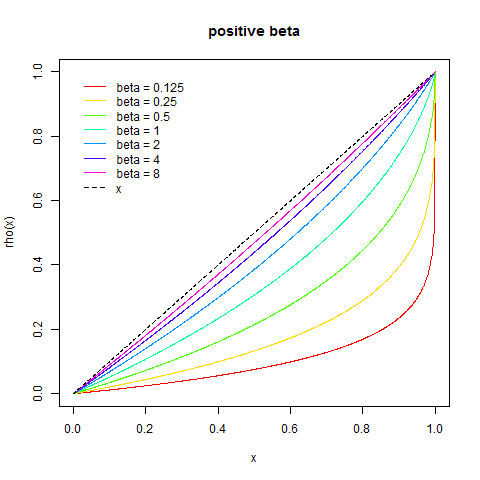
\includegraphics[width=0.6\textwidth]{fig/yule-beta.png}
	\end{center}
	\caption{Yule過程の解}\label{fig:Yule過程の解}
\end{figure} %}

\begin{todo}[今後の予定]\label{todo:今後の予定} %{
	メモ
	\begin{description} %{
		\item[2015-01-26] $\rho(\beta|x)$と$\CDF$(累積確率密度分布)との関係
		を調べる。少なくとも、$\rho(\beta|1)=\CDF(1)$となる。
		\item[2015-01-26] $\rho(\beta|-)$の逆関数を求める。
		$\rho(\beta|-):[0,1]\to[0,1]$は$1:1$になっているので、Lagrangeの定理を
		使って逆関数が求められる。
		\item[2015-01-26] $\rho(\beta|x)$の$x$についての解析接続を調べる。
		今のところ、優先順位は低い。
		\item[2015-01-25] $\beta\to\infty$の被積分関数の局在化によって説明する。
		\begin{description} %{
			\item[2015-01-26] 終了
		\end{description} %}
		\item[2015-01-25] ジーナスの確率分布$\rho(t,x)$ではなく分布そのもの
		$\nu(t,x)$を扱うことができないだろうか?
	\end{description} %}
	\EOP
\end{todo} %todo:今後の予定}
\subsection{微分方程式の解}\label{s2:微分方程式の解} %{
微分方程式\eqref{eq:diff-rho}をもう少し詳しく見る。

\subsubsection{線形の微分方程式}\label{s3:線形の微分方程式} %{
ゲージ変換を明示するために$\fukuso\pplr{x}$係数の$N$次元ベクトルで考える。

行列$A(x)\in M_N\plra{\fukuso\pplr{x}}$とベクトル$F(x)\in \fukuso\pplr{x}^N$
を固定して、次の微分方程式を考える。
\begin{equation*}\label{eq:diff-gen}
	\clD_A\phi(x) = F(x)
	\quad\text{where}\quad \clD_A\psi(x) := \plrg{\partial_x + A(x)}\psi(x)
	\quad\text{for all } \psi(x)\in\fukuso\pplr{x}^N
\end{equation*}
任意の$U(x)\in \GL_N\plra{\fukuso\pplr{x}}$と$\phi\in\fukuso\pplr{x}^N$に
対して次のゲージ変換が成り立つ。
\begin{equation*}
	\clD_A\phi(x) = \clD_AUU^{-1}\phi(x) = U\clD_{\clD_AU}U^{-1}\phi(x)
\end{equation*}
ここで、$\clD_AU$は次のように定義する。
\begin{equation*}
	\clD_AU(x) := U^{-1}(x)\plrg{\partial_x + A(x)}U(x)
	\quad\text{for all } U(x)\in \GL_N\plra{\fukuso\pplr{x}}
\end{equation*}
したがって、$D_AG=0$となる$G(x)\in \GL_N\plra{\fukuso\pplr{x}}$が求まると、
微分方程式\eqref{eq:diff-gen}の解$\phi$が次のように求まる。
\begin{equation*}
	\phi(x, y) = G(x)\int_y^x dz G^{-1}(z)F(z)
	\implies \plrgg{\partial_x + A(x)}\phi(x, y) = F(x)
\end{equation*}
そのような$G$があれば、次の式が成り立つ。
\begin{equation*}
	D_AG(x) = 0 \iff 
	A(x) = - \plrg{\partial_xG(x)}G^{-1}(x) = G(x)\partial_xG^{-1}(x)
\end{equation*}

$N=1$の場合は、ある$0<r\in\jitu$があって、$A(x)$が$\Ballx{x_0}{r}$で正則で
あれば、任意の$x\in\Ballx{x_0}{r}$に対して次のように書ける。
\begin{equation*}
	G(x) := G(x, x_0) = \exp\plra{- \int_{x_0}^x dzA(z)}
	\quad\text{for all } x\in\Ballx{x_0}{r}
	\quad\text{when } N = 1 
\end{equation*}
%s3:線形の微分方程式}
\subsubsection{微分方程式の解}\label{s3:微分方程式の解} %{
微分方程式\eqref{eq:diff-rho}を前節\ref{s3:線形の微分方程式}の筋書きに
添って解く。

\eqref{eq:diff-rho}の両辺を$\beta x(1 - x)$で割って次のように書き直すと、
\begin{equation}\label{eq:diff-rho-1}
	\plra{\partial_x + \frac{\beta}{x(1 - x)}}\rho(x) = \frac{\beta}{1 - x}
\end{equation}
$\frac{\beta}{x(1 - x)}$がゲージ場になることがわかる。そこで、$A$を
次のようにおき、
\begin{equation*}
	A(x) := \frac{\beta}{x(1 - x)}
\end{equation*}
\eqref{eq:diff-rho-1}の右辺が$xA(x)$と書けることに注意すると、
\eqref{eq:diff-rho-1}は次のように書け、
\begin{equation*}
	\plrg{\partial_x + A(x)}\rho(x) = xA(x)
\end{equation*}
その解$\rho(\beta|x,y)$は次のように書ける。
\begin{equation}\begin{split}\label{eq:rho-int-a}
	\rho(\beta|x,y) &= \exp\plra{- \int_{x_0}^x ds A(s)}
		\int_y^x dz \exp\plra{\int_{x_0}^z ds A(s)}zA(z) \\
	&= \exp\plra{- \int_{x_0}^x ds A(s)}
		\int_y^x dz \plra{\partial_z\exp\plra{\int_{x_0}^z ds A(s)}}z \\
\end{split}\end{equation}
そして、ゲージ場の積分は次のようになり、
\begin{equation*}
	\int_{x_0}^z ds A(s) = \int_{x_0}^z ds \frac{\beta}{x(1 - x)} 
	= \beta\ln\frac{\sigma(x)}{\sigma(x_0)}
\end{equation*}
解は次の形にまとまる。
\begin{equation*}
	\rho(\beta|x,y) = \int_{z=y}^x d\plra{\frac{\sigma(z)}{\sigma(x)}}^\beta z
\end{equation*}
ここで、$\sigma$は$(0,1,\infty)$を$(0,\infty,-1)$に移すM\"obius変換で、
次のように定義する。
\begin{equation*}
	\sigma(x) := \frac{x}{1 - x}
\end{equation*}
$\sigma(x)^\beta$は、$x=0$に$\beta$次のゼロ点、$x=1$に$\beta$次の発散点を
持つ。このことは、$D_\beta$の特異点が、確定特異点の$\set{0,1}$だけに
なっていることを反映している。任意の$0<\beta$に対して$x=0$で正則となることを
要請すると、$x=0$で$1/\sigma(x)$から生じる発散を避けるために、積分の始点$y$
が$0$に定まる。
\begin{equation}\label{eq:rho-int-1}
	\rho(\beta|x) := \rho(\beta|x,0) 
	= \int_{z=0}^x d\plra{\frac{\sigma(z)}{\sigma(x)}}^\beta z
\end{equation}
この解は次の性質を満たす。

\begin{description} %{
	\item[ベータ関数] 任意の$x\in\jitu$に対して$\rho(0|x)=0$だから、
	$0<\beta$の場合を考える。この時、\eqref{eq:rho-int-1}の積分変数を
	次のように変換していく。
	\begin{alignat*}{2}
		\rho(\beta|x) 
		&= \int_0^1 ds^\beta \sigma^{-1}\plrg{\sigma(x)s}
		&\quad&\text{// } s = \frac{\sigma(z)}{\sigma(x)} \\
		&= \beta x\int_0^1 ds \frac{s^\beta}{1 - x(1 - s)} \\
		&= \beta x\int_0^1 dt \frac{(1 - t)^\beta}{1 - xt}
		&\quad&\text{// } t = 1 - s
	\end{alignat*}
	この式では$\rho(0|x)=0$となるから、$\beta=0$の時も成り立ち、
	\begin{equation}\label{eq:rho-int-beta}
		\rho(\beta|x) = \beta x\int_0^1 dt \frac{(1 - t)^\beta}{1 - xt}
		\quad\text{for all } x < 1,\; 0 \le \beta
	\end{equation}
	原点近傍で次の級数展開が成り立つ。
	\begin{equation}\label{eq:rho-beta}
		\rho(\beta|x) = \beta x\sum_{n\in\sizen} x^nB(n + 1, \beta + 1)
		\quad\text{for all } |x| < 1 ,\; 0 \le \beta
	\end{equation}
	%
	\item[$x=0$の近傍] $x=0$近傍の様子は、級数展開\eqref{eq:rho-tay-beta}
	によってわかる。
	%
	\item[$x=1$の近傍] 積分表示\eqref{eq:rho-int-beta}から、$\rho(\beta|1)$が
	次のようになることがわかる。
	\begin{equation*}
		\rho(\beta|1) = \beta\int_0^1 dt (1 - t)^{\beta - 1}
		= \begin{cases}
			0, &\text{ if } \beta = 0 \\
			1, &\text{ otherwise } \\
		\end{cases}
	\end{equation*}
	また、\eqref{eq:rho-int-beta}を次のように書き換えると、
	\begin{equation*}
		\rho(\beta|x) = - \beta\int_{t=0}^1 d\plrg{\ln(1 - xt)}(1 - t)^\beta
	\end{equation*}
	任意の$n\in\sizen_+$に対して次の式を得る。
	\begin{equation*}
		\partial_x^n\rho(\beta|x) = \beta\int_{t=0}^1 
			d\plra{\frac{t}{1 - xt}}^n(1 - t)^\beta
	\end{equation*}
	この式を部分積分すると、$\partial_x^n\rho(\beta|x=1)$が次のようになること
	がわかる。
	\begin{equation*}\begin{split}
		\partial_x^n\rho(\beta|x=1)
		&= \beta \lim_{t\to1} t(1 - t)^{\beta - n}
			+ \beta^2\int_0^1 dt t^n(1 - t)^{\beta - n - 1} \\
		&= \begin{cases}
			B(n + 1, \beta - n), &\text{ if } n < \beta \\
			\infty, &\text{ otherwise } \\
		\end{cases}
	\end{split}\end{equation*}
	%
	\item[$\beta=0$の極限] $\beta=0$の時は、任意の$x\in\jitu$に対して
	$\rho(0|x)=0$となる。一方、任意の$0<\beta$で$\rho(\beta|1)=1$だから、
	$\lim_{\beta\to0+0}\rho(\beta|1)\neq\rho(0|1)$となって、$\rho(\beta|x)$は
	$\beta$について$0$で不連続になる。
	%
	\item[$\beta=\infty$の極限] 積分表示\eqref{eq:rho-int-beta}で、$\beta$が
	無限大に近づくと、被積分関数が局在化する。
	\begin{equation*}
		\lim_{\beta\to\infty}(1 - t)^\beta = \begin{cases}
			1, &\text{ if } t = 0 \\
			0, &\text{ otherwise } \\
		\end{cases}
	\end{equation*}
	このことは、部分積分を使って、次のように表され、
	\begin{equation*}\begin{split}
		\rho(\beta|x) &= \beta\int_0^1 dt\frac{(1 - t)^\beta}{1 - xt}
		= - \frac{\beta x}{\beta + 1}\blra{\frac{(1 - t)^{\beta + 1}}{1 - xt}}
			+ \frac{\beta x}{\beta + 1}\int_0^1 dt (1 - t)^{\beta + 1}
			\partial_x\frac{t}{1 -xt} \\
		&= \frac{\beta x}{\beta + 1} + \bigO\frac{x^2}{\beta}
	\end{split}\end{equation*}
	任意の$0\le x\le 1$で$\rho(\infty|x) = x$となることがわかる。
	この$\beta\to\infty$の漸近形は、固定した$x$と大きな$y$に対して成り立つ
	ベータ関数の近似$B(x,y)\sim \Gamma(x)y^{-x}$を\eqref{eq:rho-beta}に適用
	しても得られる。
	\begin{equation*}
		\rho(\beta|x) = \beta\sum_{n\in\sizen} B(n + 1, \beta + 1)x^{n+1}
		\xto{\beta\to\infty} \sum_{n\in\sizen}\frac{n!x^{n + 1}}{\beta^n}
	\end{equation*}
\end{description} %}
%s3:微分方程式の解}
%s2:微分方程式の解}
%s1:Yule過程}
